\begin{center}
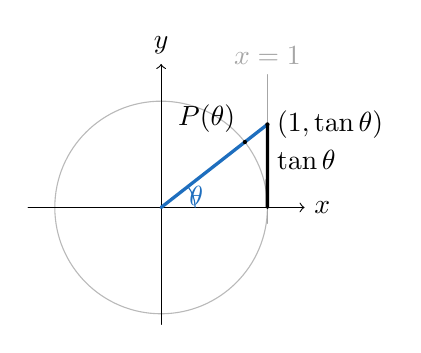
\begin{tikzpicture}[scale=1.35, line cap=round, line join=round]
  \definecolor{trigblue}{RGB}{30,110,190}
  \coordinate (O) at (0,0);
  \coordinate (P) at (38:1);
  \coordinate (T) at (1,{tan(38)});
  \draw[gray!55] (O) circle (1);
  \draw[->] (-1.25,0)--(1.35,0) node[right] {$x$};
  \draw[->] (0,-1.1)--(0,1.35) node[above] {$y$};
  \draw[gray!70] (1,-0.15)--(1,1.25) node[above] {$x=1$};
  \draw[very thick, trigblue] (O)--(T);
  \draw[very thick] (1,0)--(T);
  \fill (P) circle (0.02) node[above left] {$P(\theta)$};
  \fill (T) circle (0.02) node[right] {$(1,\tan\theta)$};
  \node[right] at (1,0.45) {$\tan\theta$};
  \draw[trigblue] (0.32,0) arc[start angle=0,end angle=38,radius=0.32];
  \node[trigblue] at (0.33,0.11) {$\theta$};
\end{tikzpicture}
\end{center}
